\section{Recap}

\begin{frame}[fragile]\frametitle{R syntax - \texttt{glm()} vs \texttt{glm()}}
  \begin{itemize}
  \item the \texttt{glm()} function needs
    \begin{itemize}
    \item a model formula (like \texttt{lm})
    \item the specification of error distribution (\texttt{family=})
    \end{itemize}
  \end{itemize}
\begin{exampleblock}{Input/Output}\small
\begin{verbatim}
> m1 <- lm(bweight ~ hyp, data=births)
> m2 <- glm(bweight ~ hyp, family=gaussian, data=births)
\end{verbatim}
\end{exampleblock}
\end{frame}

\begin{frame}\frametitle{\texttt{glm()} for logistic regression}
  \begin{itemize}
    \item every error family has a canonical link
    \item we have seen binomial error family with its canonical logit link
    \item common choices for link functions used with binomial errors
      \begin{itemize}
      \item logit: $\eta = \log(p/(1-p))$
      \item probit: $\eta = \Phi^{-1}(p)$ 
      \item log-log: $\log(-\log(1-p))$
      \end{itemize}
  \end{itemize}
\end{frame}


\begin{frame}\frametitle{Odds}
  \begin{itemize}
    \item logistic regression is more understandable if you look at the coefficients in terms of odds where
    \item $\Omega(A) = \frac{P(A)}{1-P(A)}$
    \item so what are the corresponding odds for a probability of
      \begin{itemize}
      \item $p = 1$
      \item $p = 0.99$
      \item $p = 0.5$
      \item $p = 0.1$
      \item $p = 0.01$
      \item $p = 0$        
      \end{itemize}
  \end{itemize}
\end{frame}


\begin{frame}\frametitle{Odds}
\begin{columns}
  \begin{column}{0.4\textwidth}
    $$p = 1$$
    $$p = 0.99$$
    $$p = 0.5$$
    $$p = 0.1$$
    $$p = 0.01$$
    $$p = 0$$    
  \end{column}
  \begin{column}{0.4\textwidth}
    $$\omega = \infty$$
    $$\omega = 99$$
    $$\omega = 1$$
    $$\omega = 0.\bar{1}$$
    $$\omega = 0.\overline{01}$$
    $$\omega = 0$$
  \end{column}
\end{columns}
\end{frame}


\begin{frame}[fragile]\frametitle{Remember the Data}
\footnotesize
\begin{exampleblock}{Input/Output}
\begin{semiverbatim}
  > str(births)
  'data.frame':	500 obs. of  8 variables:
 $ id     : num  100 101 102 103 104 105 106 107 108 109 ...
 $ preterm: Factor w/ 2 levels "preterm","normal": 2 2 2 2 2 2 2 NA 2 2 ...
 $ gestwks: num  39.8 39 38.1 39.5 39.5 ...
 $ hyp    : Factor w/ 2 levels "normal","hyper": 1 1 1 1 2 1 2 1 1 1 ...
 $ matage : num  33 32 33 38 40 29 32 40 41 39 ...
 $ bweight: num  3576 3784 2796 3226 3138 ...
 $ lowbw  : Factor w/ 2 levels "normal","low": 1 1 1 1 1 1 1 1 1 1 ...
 $ sex    : Factor w/ 2 levels "M","F": 2 2 2 2 2 2 1 1 2 2 ...
\end{semiverbatim}
\end{exampleblock}
Data from: Michael Hills and Bianca De Stavola (2002). A Short Introduction
     to Stata 8 for Biostatistics, Timberlake Consultants Ltd URL:
     http://www.timberlake.co.uk
\end{frame}

\begin{frame}[fragile]\frametitle{Exercises}
Remember: We used hypertension of the mom to explain variation in the birth weight of the kid. Without looking in the material of the last session, try to redo the model. Here are some hints:
\begin{itemize}
\item of course you need the \texttt{glm()} function
\item you need to specify the formula which has to have the general form $y \sim x$
\item additional you need to specify the data and the error family (in the case \texttt{binomial})
\item use the \texttt{summary()} function on the model
\item use \texttt{Effects()} or \texttt{allEffects()} commands on the model
\item how to interpret the results? Is the effect of hypertension statistically significant?
\end{itemize}
\end{frame}


\begin{frame}[fragile]\frametitle{Exercise - Solution}\footnotesize
\begin{exampleblock}{Input/Output}\scriptsize
\begin{verbatim}
> m <- glm(lowbw ~ hyp, family=binomial, data=births)
> summary(m)
Call:
glm(formula = lowbw ~ hyp, family = binomial, data = births)

Deviance Residuals: 
    Min       1Q   Median       3Q      Max  
-0.8067  -0.4430  -0.4430  -0.4430   2.1773  

Coefficients:
            Estimate Std. Error z value Pr(>|z|)    
(Intercept)  -2.2721     0.1661 -13.682  < 2e-16 ***
hyphyper      1.3166     0.3111   4.232 2.32e-05 ***
---

(Dispersion parameter for binomial family taken to be 1)

    Null deviance: 366.92  on 499  degrees of freedom
Residual deviance: 350.84  on 498  degrees of freedom
AIC: 354.84

\end{verbatim}
\end{exampleblock}
\end{frame}



\begin{frame}[fragile]\frametitle{Exercise - Solution}\footnotesize
\begin{exampleblock}{Input/Output}\small
\begin{verbatim}
> require(effects)
Lade nötiges Paket: effects
> allEffects(m.hyp)
 model: lowbw ~ hyp

 hyp effect
hyp
    normal      hyper 
0.09345794 0.27777778 
> plot(allEffects(m.hyp))
\end{verbatim}
\end{exampleblock}
\end{frame}



\begin{frame}[fragile]\frametitle{Exercise - Solution}\footnotesize
  \begin{center}
    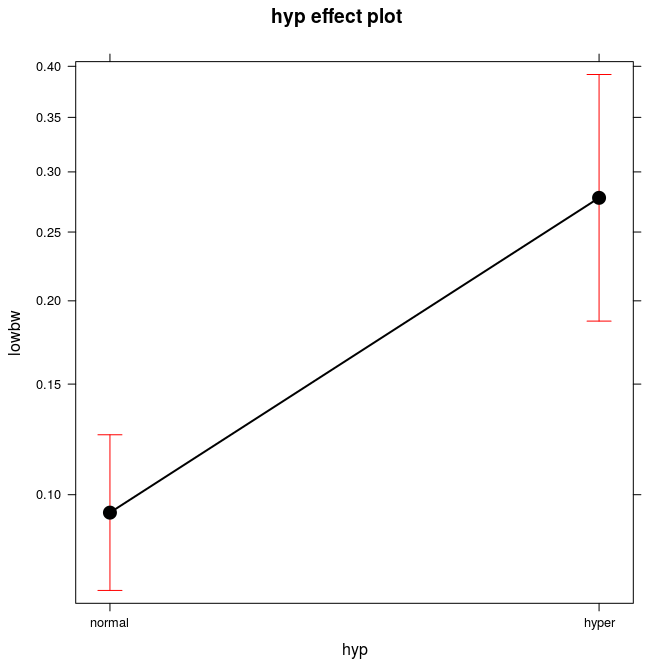
\includegraphics[width = 8cm]{hypeffect.png}
  \end{center}

\end{frame}

\begin{frame}[fragile]\frametitle{Exercise - Solution}\footnotesize
\begin{exampleblock}{Input/Output}\scriptsize
\begin{verbatim}
> res <- allEffects(m.hyp, se = T)
> summary(res)
 model: lowbw ~ hyp

 hyp effect
hyp
    normal      hyper 
0.09345794 0.27777778 

 Lower 95 Percent Confidence Limits
hyp
    normal      hyper 
0.06929267 0.18675845 

 Upper 95 Percent Confidence Limits
hyp
   normal     hyper 
0.1249195 0.3917861 
\end{verbatim}
\end{exampleblock}
\end{frame}

\begin{frame}[fragile]\frametitle{Exercises}
  What is the relationship between the coefficients of the model (from the model summary) and the effects?
\end{frame}


\begin{frame}[fragile]\frametitle{Exercises - Solutions}
  What is the relationship between the coefficients of the model (from the model summary) and the effects?
  \begin{itemize}
  \item we have to use the inverse link function on the coefficients to transform the coefficients on the logit scale to more interpretable probabilities
  \end{itemize}
  \begin{exampleblock}{Input/Output}
\begin{verbatim}
> invlogit(coef(m.hyp)[1])
(Intercept) 
 0.09345794 
> invlogit(coef(m.hyp)[1] + coef(m.hyp)[2])
(Intercept) 
  0.2777778 
\end{verbatim}
  \end{exampleblock}
  \begin{itemize}
\item 
\end{itemize}
\end{frame}


\section{Binomial/Logistic Regression}

\begin{frame}[fragile]\frametitle{Simple Logistic Regression}
\begin{itemize}
\item now we model the probability of low birth weight dependent on gestational age (numeric variable)
\item so the model in R is 
  \begin{exampleblock}{Input}\footnotesize
\begin{verbatim}
> m.wks <- glm(lowbw ~ gestwks, family=binomial, data=births)
\end{verbatim}
  \end{exampleblock}\normalsize
\item and as math formula
$$ \log\left(\frac{\mbox{Pr(lowbw)}}{1-\mbox{Pr(lowbw)}}\right) = \beta_0 + \beta_1 \cdot \mbox{gestwks} + \epsilon$$
\end{itemize}
\end{frame}


\begin{frame}[fragile]\frametitle{Simple Logistic Regression}
\begin{itemize}
\item where the output look similar to the output above
  \begin{exampleblock}{Input/Output}\scriptsize
\begin{verbatim}
> summary(m.wks)

Call:
glm(formula = lowbw ~ gestwks, family = binomial, data = births)

Deviance Residuals: 
    Min       1Q   Median       3Q      Max  
-2.0873  -0.3623  -0.2223  -0.1369   2.9753  

Coefficients:
            Estimate Std. Error z value Pr(>|z|)    
(Intercept)  31.8477     4.0574   7.849 4.18e-15 ***
gestwks      -0.8965     0.1084  -8.272  < 2e-16 ***
---
Signif. codes:  0 ‘***’ 0.001 ‘**’ 0.01 ‘*’ 0.05 ‘.’ 0.1 ‘ ’ 1

(Dispersion parameter for binomial family taken to be 1)

    Null deviance: 360.38  on 489  degrees of freedom
Residual deviance: 205.75  on 488  degrees of freedom
  (10 observations deleted due to missingness)
AIC: 209.75

Number of Fisher Scoring iterations: 6
\end{verbatim}
  \end{exampleblock}
\end{itemize}
\end{frame}


\begin{frame}[fragile]\frametitle{Understanding the Coefficients}
\begin{itemize}
\item this relationship is described by $$\mbox{Pr(lowbw)}=\mbox{logit}^{-1}(31.8477 + -0.8965 \cdot \mbox{gestwks}) $$
\item the intercept
  \begin{exampleblock}{Input/Output}
\begin{verbatim}
> invlogit(coef(m.wks)[1])
(Intercept) 
  1
\end{verbatim}
  \end{exampleblock}
is interpretable as the probability for a low birth weight at a hypothetical gestational age of 0 (which makes no sense because it lies outside the range of gestational ages in our data and is nonsense anyway)
\item the parameter for \texttt{gestwks} describes how fast the probability decreases with increasing gestational age
\end{itemize}
\end{frame}

\begin{frame}[fragile]\frametitle{Understanding the Coefficients}
$$\mbox{Pr(lowbw)}=\mbox{logit}^{-1}(31.8477 + -0.8965 \cdot \mbox{gestwks}) $$
\begin{itemize}
\item the coefficient for \texttt{gestwks} is best interpretable if we use it as argument to the exponential function
  \begin{exampleblock}{Input/Output}
\begin{verbatim}
> exp(coef(m.wks)[2])
  gestwks 
0.4080114 
\end{verbatim}
  \end{exampleblock}
this way it is interpretable as odds ratio for low birth weight for a difference of 1 week of gestational age (because we are measuring gestational in weeks as unit)
\end{itemize}
\end{frame}


\begin{frame}[fragile]\frametitle{Exercise}
  \begin{enumerate}
  \item here is a example for the \texttt{Effects()} command for regression
    \begin{exampleblock}{Input/Output}\scriptsize
\begin{verbatim}
> Effect("gestwks",m.wks)

 gestwks effect
gestwks
        25         30         35         40 
0.99992022 0.99299324 0.61574996 0.01779725 
> Effect("gestwks",m.wks,xlevels = list(gestwks = c(20,30,40)))

 gestwks effect
gestwks
        20         30         40 
0.99999910 0.99299324 0.01779725   
\end{verbatim}
    \end{exampleblock}\normalsize
\item use the command to gain the estimated probability of low birth weight for a gestational age of 27 and 36 weeks
  \end{enumerate}
\end{frame}


\begin{frame}[fragile]\frametitle{\texttt{ggplot()} and \texttt{glm()}}
  \begin{itemize}
  \item ggplot2 knows also glms
  \item unfortunately the y-variable needs to be coded in 0s and 1s, but we can do this on the fly with \texttt{as.numeric()}
  \end{itemize}
  \begin{exampleblock}{Input}\scriptsize
\begin{verbatim}
> require(ggplot2)
> ggplot(births,aes(x = gestwks, y = as.numeric(lowbw)-1)) +
+     geom_smooth(method = "glm", family = "binomial",se = F,size = 2) +
+     geom_point(shape="|")  ## adds actual values  
\end{verbatim}
  \end{exampleblock}
\end{frame}


\begin{frame}\frametitle{\texttt{ggplot()} and \texttt{glm()}}
  \begin{center}
    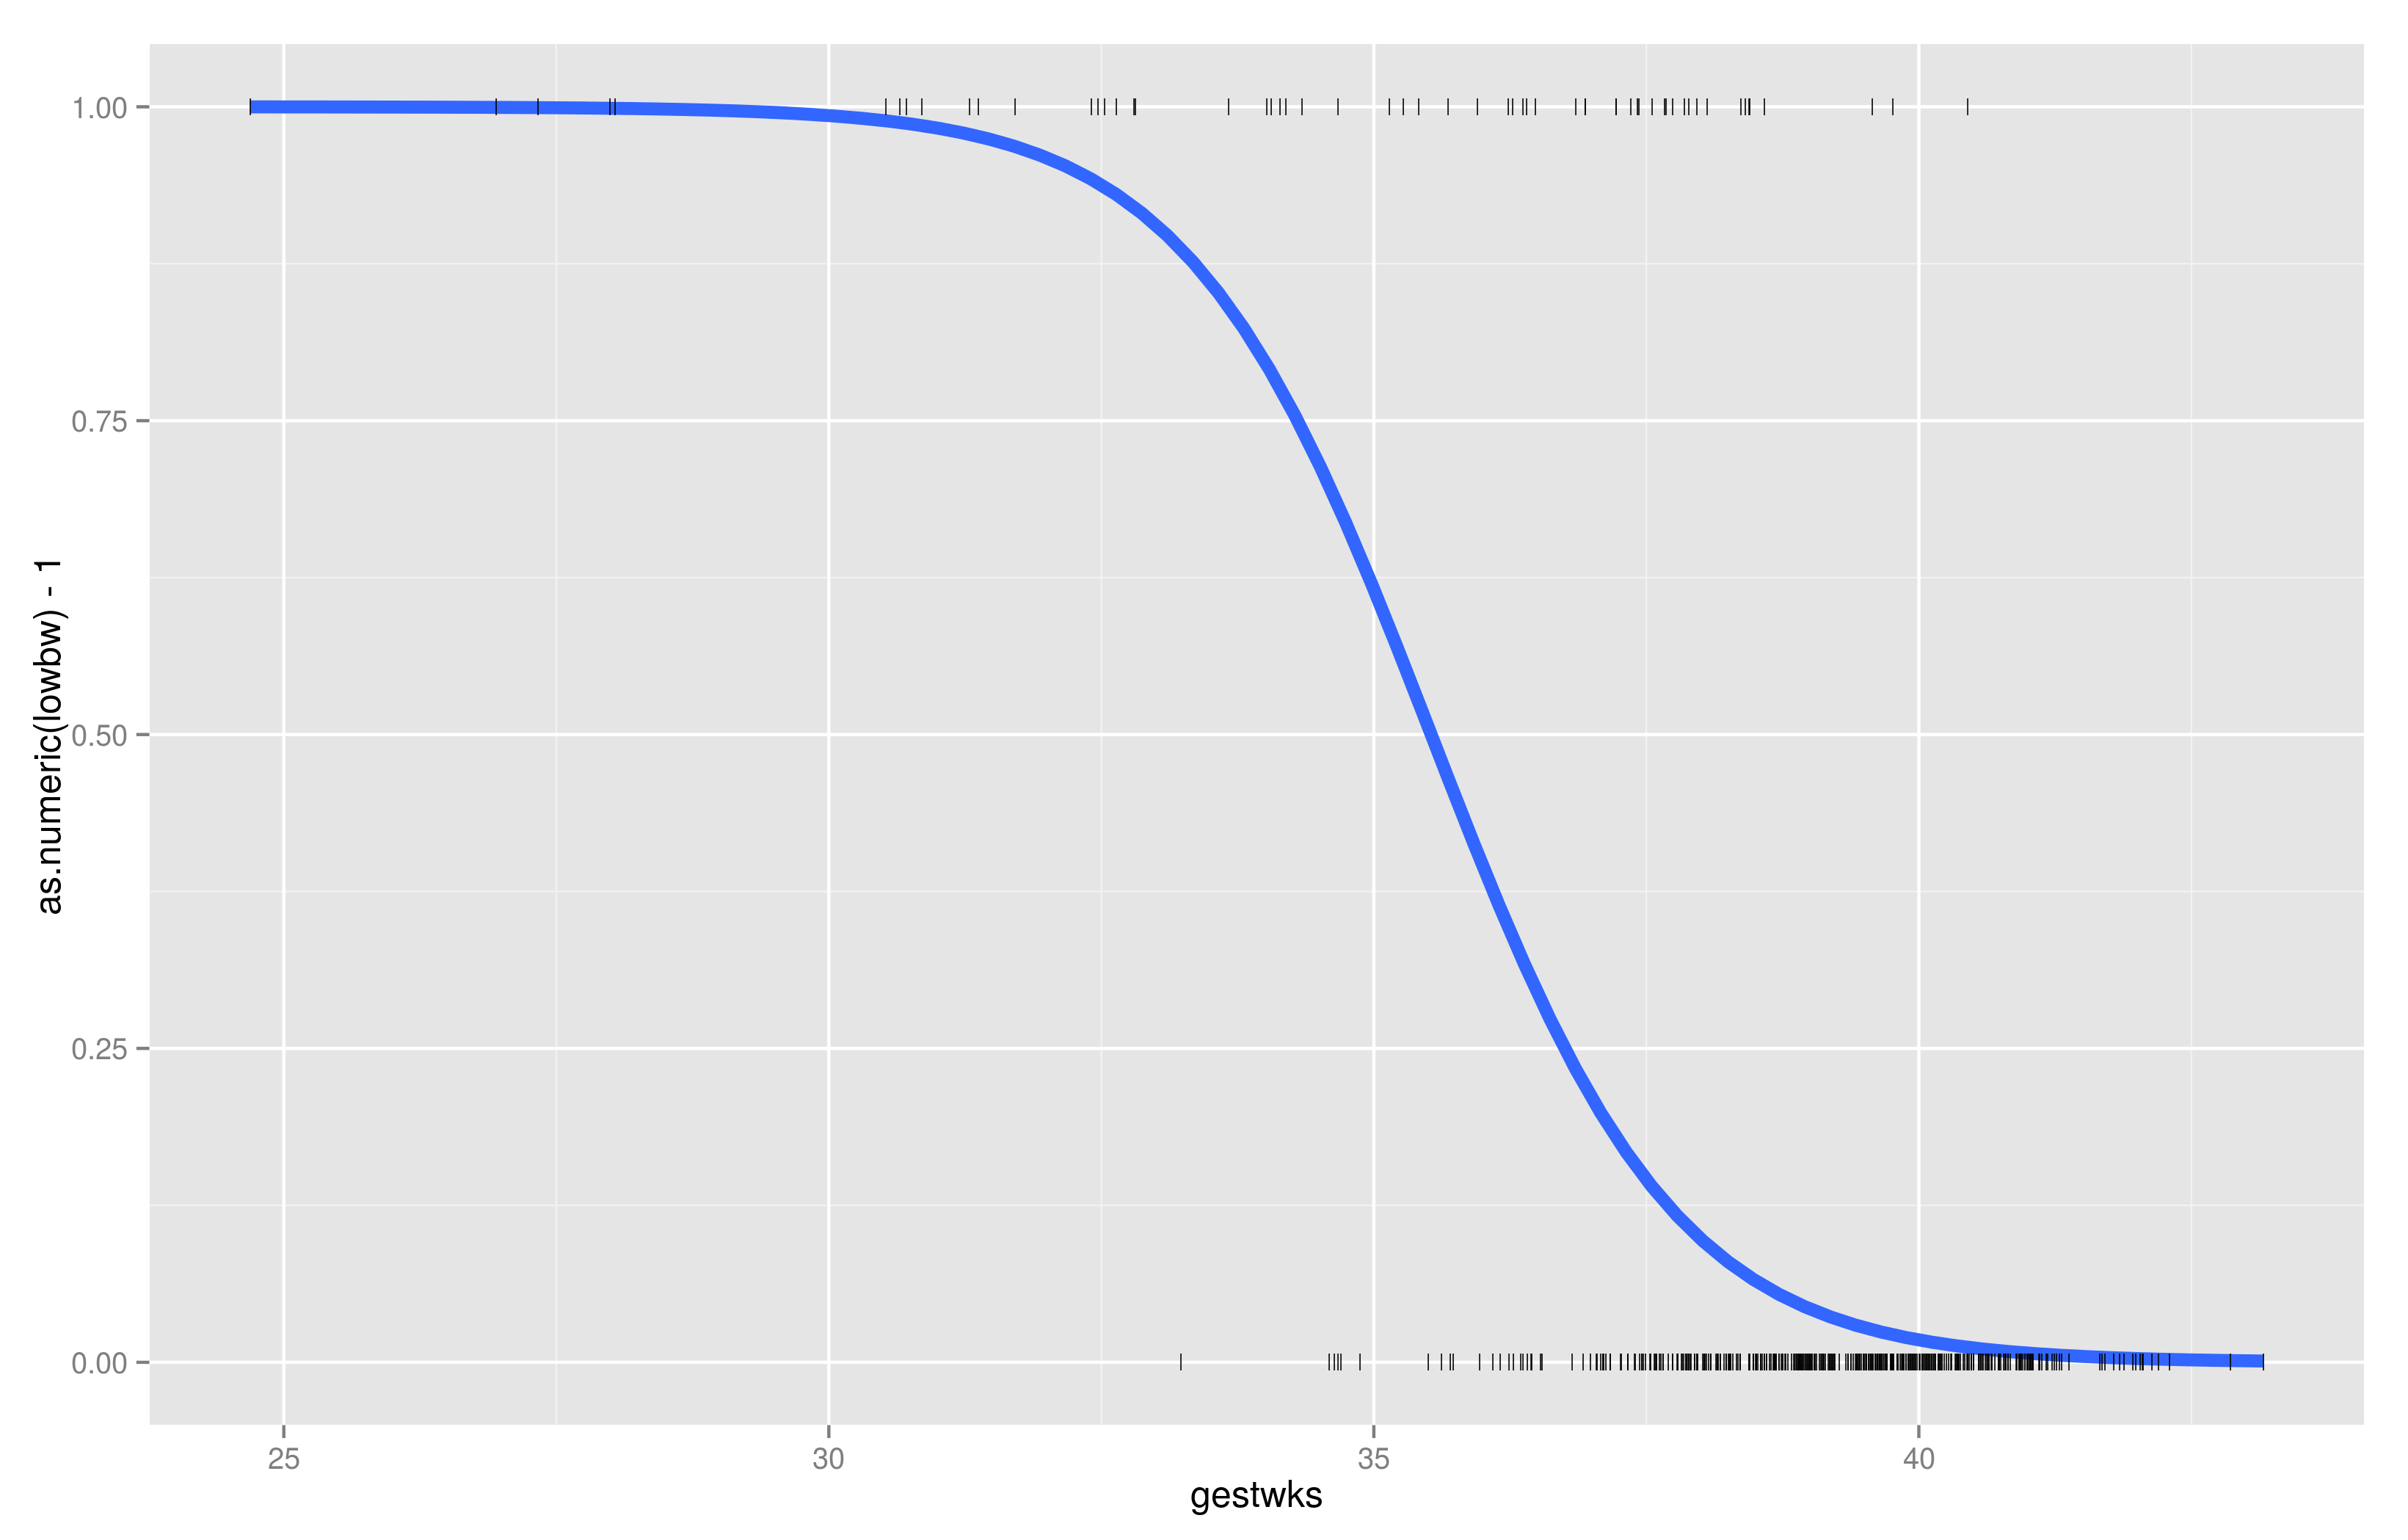
\includegraphics[width=11cm]{glmggplot.png}
  \end{center}
\end{frame}


\begin{frame}[fragile]\frametitle{Exercise}
Take the code producing the graph
  \begin{enumerate}
  \item try to change the axis titles (\texttt{xlab()} and \texttt{ylab()})
  \item add a title (\texttt{ggtitle()})
  \item change the colour of the function to black, set se = T
  \item change the colour of the points to red for the low birth weight and green for the one with normal birth weight
  \item change the position of the legend; place it somewhere near the upper right corner inside the plotting area (\texttt{legend.position})
  \end{enumerate}
\end{frame}

\section{The famous O-Ring example}

\begin{frame}[fragile]\frametitle{The Challenger Disaster Example}
In January 1986, the space shuttle Challenger exploded shortly after launch. An
investigation was launched into the cause of the crash and attention focused on the rubber
O-ring seals in the rocket boosters. At lower temperatures, rubber becomes more brittle
and is a less effective sealant. At the time of the launch, the temperature was 31\degree F. Could
the failure of the O-rings have been predicted? In the 23 previous shuttle missions for
which data exists, some evidence of damage due to blow by and erosion was recorded on
some O-rings. Each shuttle had two boosters, each with three O-rings. For each mission,
we know the number of O-rings out of six showing some damage and the launch
temperature.(faraway)

\url{http://www.history.com/topics/challenger-disaster/videos/engineering-disasters---challenger}

\end{frame}

\begin{frame}[fragile]\frametitle{The Challenger Disaster Example}
\begin{itemize}
\item the data are given in the data frame \texttt{orings} in the \texttt{faraway} package
\item after loading we have a look at the first six lines
  \begin{exampleblock}{Input/Output}\small
\begin{verbatim}
> library(faraway)
> data(orings)
> head(orings)
  temp damage
1   53      5
2   57      1
3   58      1
4   63      1
5   66      0
6   67      0
\end{verbatim}
  \end{exampleblock}

\item we see that every shuttle mission has its own row (but not every O-ring)
\end{itemize}
\end{frame}

\begin{frame}[fragile]\frametitle{The Challenger Disaster Example}
\begin{itemize}
\item that is not a problem: one way of defining a binary response variable in a glm is to form a two-column matrix with the first
column representing the number of “successes” y and the second column the number of “failures” n–y.
\begin{exampleblock}{Input/Output}\small
\begin{verbatim}
> m.oring <- glm(cbind(damage,6-damage) ~ temp,
+                      family=binomial, orings)
\end{verbatim}
\end{exampleblock}

\normalsize
\end{itemize}
\end{frame}

\begin{frame}[fragile]\frametitle{The Challenger Disaster Example}
\begin{itemize}
\item the output looks familiar:
  \begin{exampleblock}{Input/Output}\scriptsize
\begin{verbatim}
> summary(m.oring)
Call:
glm(formula = cbind(damage, 6 - damage) ~ temp, 
     family = binomial, data = orings)
Deviance Residuals: 
    Min       1Q   Median       3Q      Max  
-0.9529  -0.7345  -0.4393  -0.2079   1.9565  
Coefficients:
            Estimate Std. Error z value Pr(>|z|)    
(Intercept) 11.66299    3.29626   3.538 0.000403 ***
temp        -0.21623    0.05318  -4.066 4.78e-05 ***
(Dispersion parameter for binomial family taken to be 1)
    Null deviance: 38.898  on 22  degrees of freedom
Residual deviance: 16.912  on 21  degrees of freedom
AIC: 33.675
\end{verbatim}
  \end{exampleblock}
\item remember, the response is a probability. Therefore our model describes the probability of a damaged O-ring depending on the temperature
\end{itemize}
\end{frame}


\begin{frame}[fragile]\frametitle{Understanding the Coefficients}
\begin{itemize}
\item this relationship is described by $$\mbox{Pr(damage)}=\mbox{logit}^{-1}(11.66299 + -0.21623 \cdot \mbox{temp}) $$
\item the intercept
  \begin{exampleblock}{Input/Output}
\begin{verbatim}
> invlogit(coef(m.oring)[1])
(Intercept) 
  0.9999914 
\end{verbatim}
  \end{exampleblock}

is interpretable as the probability for a damaged O-ring at a temperature of 0\degree F
\item the parameter for temperature describes how fast the probability decreases with increasing temperature and it is again best interpretable as odds ratio 
\end{itemize}
\begin{exampleblock}{Input/Output}\footnotesize
\begin{verbatim}
> exp(coef(m.oring)[2])
     temp 
0.8055471 
\end{verbatim}
\end{exampleblock}

\end{frame}

\begin{frame}[fragile]\frametitle{Understanding the Coefficients}\footnotesize
\begin{verbatim}

\end{verbatim}
\begin{center}
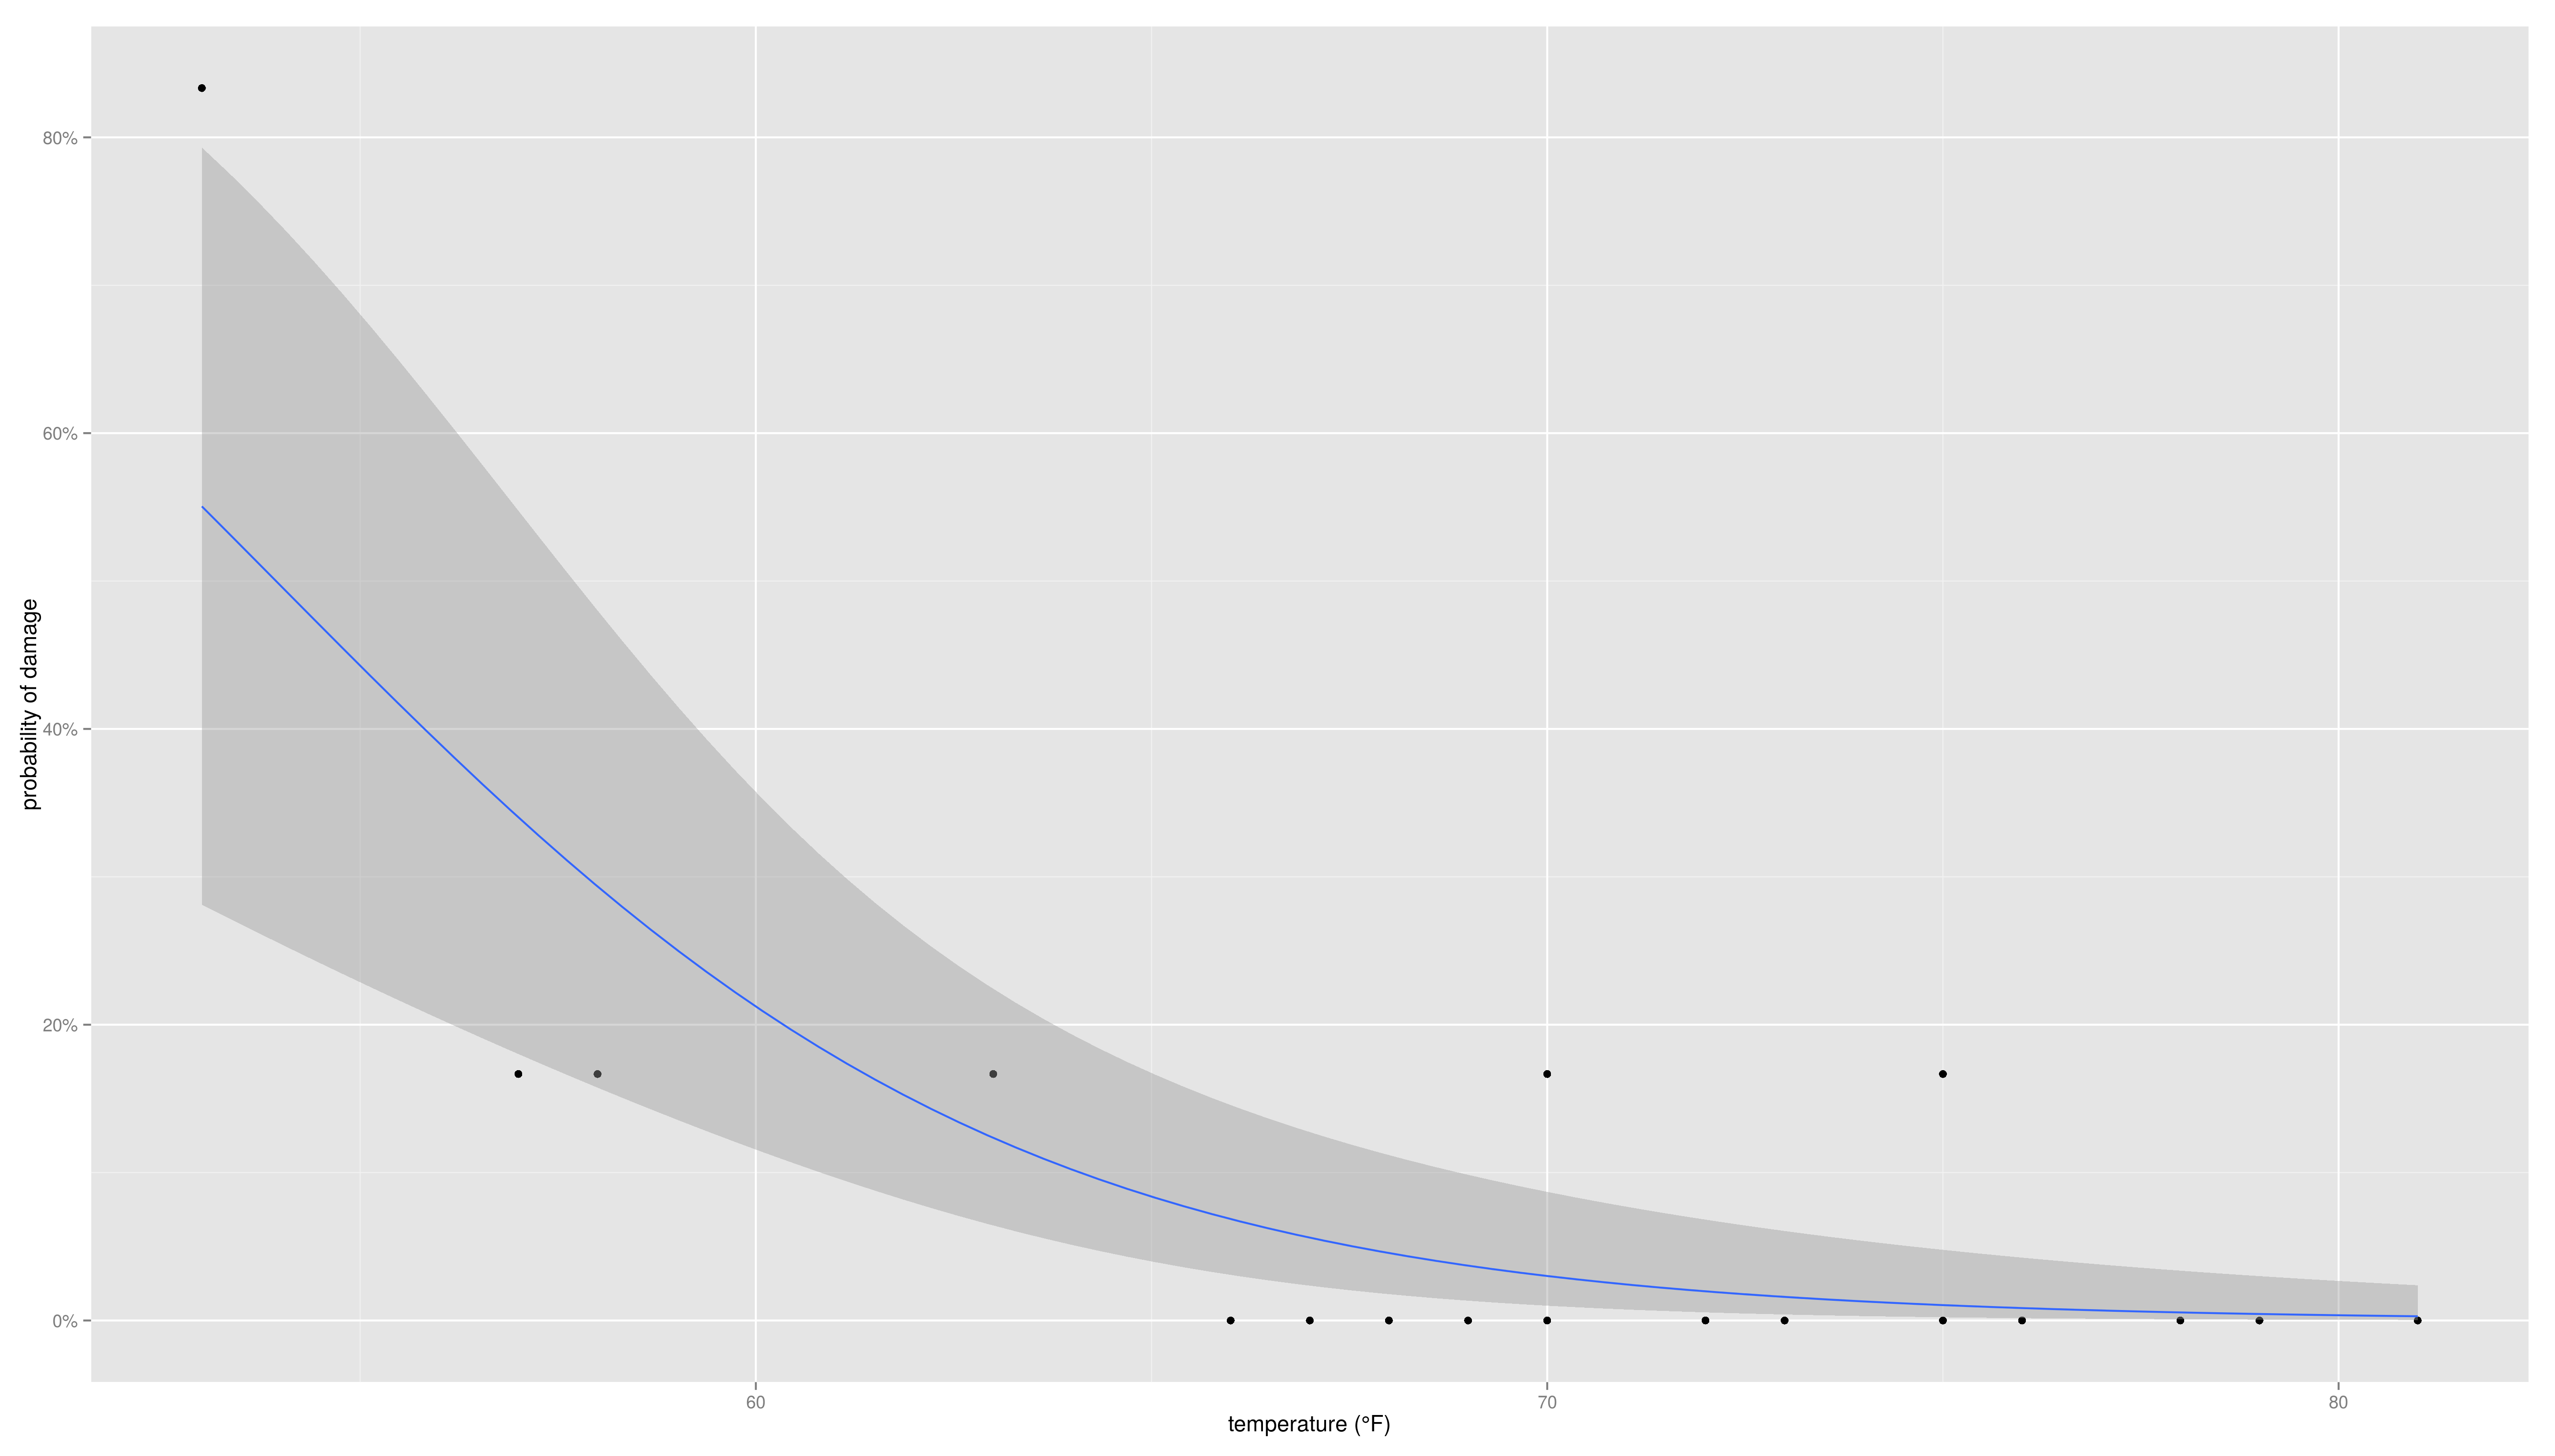
\includegraphics[width=11.5cm]{challenger.png}
\end{center}
\end{frame}

\begin{frame}[fragile]\frametitle{Understanding the Coefficients}
and the same plot made with ggplot (incl. adding a table)
\begin{center}
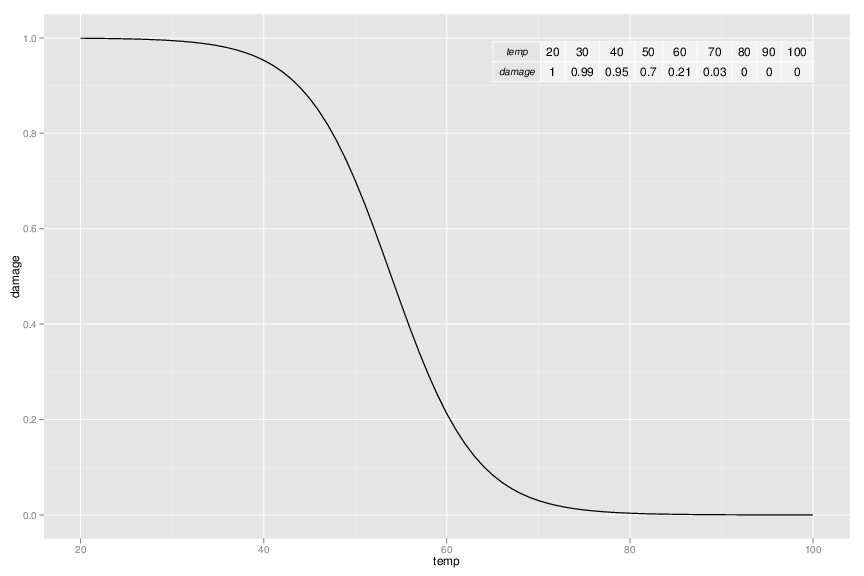
\includegraphics[width=11.5cm]{challenger2.png}
\end{center}
\end{frame}


\section[Binomial Ancova]{Ancova with a Binary Response Variable }

\begin{frame}[fragile]\frametitle{Parasite Infection Example}
\begin{itemize}
\item the binary response variable is parasite infection (infected or not) 
\item the explanatory variables are weight and age (continuous) 
\item and sex (categorical)
\item we want to investigate if there is a different effect of age for each of the sexes on the outcome variable
\end{itemize}
\begin{exampleblock}{Input/Output}\footnotesize
\begin{verbatim}
> load("infection.rdata")
> summary(infection)
         infected        age             sex     
 infected    :338   Min.   :  2.00   female:243  
 not infected:162   1st Qu.: 46.00   male  :257  
                    Median : 84.50               
                    Mean   : 93.69               
                    3rd Qu.:139.25               
                    Max.   :200.00               
\end{verbatim}
\end{exampleblock}

\end{frame}


\begin{frame}[fragile]\frametitle{Parasite Infection Example}\footnotesize
  \begin{exampleblock}{Input/Output}\scriptsize
\begin{verbatim}
> m.inf <- glm(infected~age*sex,family=binomial,
+                               data=infection)
> summary(m.inf)
Call:
glm(formula = infected ~ age * sex, family = binomial, 
                                     data = infection)
Deviance Residuals: 
    Min       1Q   Median       3Q      Max  
-2.0411  -0.7307  -0.4363   0.6632   2.3215  
Coefficients:
             Estimate Std. Error z value Pr(>|z|)    
(Intercept) -3.000513   0.413639  -7.254 4.05e-13 ***
age          0.015657   0.003176   4.929 8.25e-07 ***
sex          0.116664   0.553956   0.211   0.8332    
age:sex      0.011050   0.004612   2.396   0.0166 *  

(Dispersion parameter for binomial family taken to be 1)
    Null deviance: 629.85  on 499  degrees of freedom
Residual deviance: 477.61  on 496  degrees of freedom
AIC: 485.61
\end{verbatim}
  \end{exampleblock}

\end{frame}

\begin{frame}[fragile]\frametitle{Parasite Infection Example}
\begin{itemize}
\item so for male at a age of 0 there is a probability of
    \begin{exampleblock}{Input/Output}
\begin{verbatim}
> invlogit(coef(m.inf)[1])
(Intercept) 
 0.04740269 
\end{verbatim}
    \end{exampleblock}
  \item for females the probability at age 0 is
    \begin{exampleblock}{Input/Output}
\begin{verbatim}
> invlogit(coef(m.inf)[1]+coef(m.inf)[3])
(Intercept) 
 0.05295775 
\end{verbatim}
  \end{exampleblock}
\end{itemize}
\end{frame}


\begin{frame}[fragile]\frametitle{Compare Slopes}
\begin{itemize}
\item so what about the slope?
\item for males the underlying model is the following
$$\mbox{Pr(infection)}=\mbox{logit}^{-1}(-3.000513 + 0.015657 \cdot \mbox{age}) $$
\item for females the slope is almost twice as high
  $$\mbox{Pr(infection)}=\mbox{logit}^{-1}(-2.883849 + 0.02670685  \cdot \mbox{age}) $$
\end{itemize}
\end{frame}


\begin{frame}[fragile]\frametitle{Compare Slopes}
\begin{itemize}
\item looking at the odds ratios (which seem to be rather small)
\item for males and females:
  \begin{exampleblock}{Input/Output}\small
\begin{verbatim}
> exp(coef(m.inf)[2]) ## males
    age 
1.01578 
> exp(coef(m.inf)[2] + coef(m.inf)[4]) ## females
     age  
1.027067 
\end{verbatim}
  \end{exampleblock}
\item these are the odds ratios for +1 time unit
\end{itemize}
\end{frame}

\begin{frame}[fragile]\frametitle{Compare Slopes}
  \begin{itemize}
  \item if time unit is days you get the odds ratio for +1 month   by
  \begin{exampleblock}{Input/Output}\small
\begin{verbatim}
> exp(30 * coef(m.inf)[2])
     age 
1.599512 
> exp(30 * (coef(m.inf)[2] + coef(m.inf)[4]))
     age 
2.228225 
\end{verbatim}
  \end{exampleblock}
\item so keep in mind the scale you are measuring on
\end{itemize}
\end{frame}

  \begin{frame}[fragile]\frametitle{Compare Slopes}
\begin{itemize}
\item we can also compare them by looking at the age where the probability to be infected is 50\%
\item this is the case when $$-3.000513 + 0.015657 \cdot \mbox{age}=0$$  respectively $$-2.883849 + 0.02670685  \cdot \mbox{age}=0$$ you can do it by hand or use R
\end{itemize}
\end{frame}

\begin{frame}[fragile]\frametitle{Compare Slopes}
\begin{itemize}
\item \texttt{solve()} solves systems of linear equations in the form A*x=b, where A is the matrix of coefficients and b are the (negative) intercepts, here we have the special case with just one equation
  \begin{exampleblock}{Input/Output}\small
\begin{verbatim}
> ## male
> solve(0.015657,3.000513)
[1] 191.6404
> ## female
> solve(0.02670685,2.883849)
[1] 107.9816
\end{verbatim}
  \end{exampleblock}

\end{itemize}
\end{frame}

\begin{frame}[fragile]\frametitle{Compare Effects}
\begin{itemize}
\item you can also use the \texttt{allEffects()} function (part of the \texttt{effects} package), which give you the probabilities for being infected on several ages for both sexes
  \begin{exampleblock}{Input/Output}\scriptsize
\begin{verbatim}
> allEffects(m.inf)
 model: infected ~ age * sex

 age*sex effect
     sex
age            0          1
  2   0.04883687 0.05570148
  24  0.06756215 0.09596497
  46  0.09276694 0.16038932
  68  0.12610300 0.25582483
  90  0.16918450 0.38219715
  112 0.22322468 0.52680374
  134 0.28853152 0.66704908
  156 0.36399154 0.78286130
  178 0.44679328 0.86645480
  200 0.53265591 0.92110968
\end{verbatim}
  \end{exampleblock}

\end{itemize}
\end{frame}


\begin{frame}[fragile]\frametitle{Compare Effects}
\begin{itemize}
\item choose values of age
  \begin{exampleblock}{Input/Output}\footnotesize
\begin{verbatim}
> allEffects(m.inf,
+            xlevels = list(age = seq(0,200,by = 50)))
 model: infected ~ age * sex

 age*sex effect
     sex
age       female       male
  0   0.04740269 0.05295775
  50  0.09817379 0.17530204
  100 0.19234385 0.44690980
  150 0.34253427 0.75439251
  200 0.53265591 0.92110968
\end{verbatim}
  \end{exampleblock}

\end{itemize}
\end{frame}

\begin{frame}[fragile]\frametitle{Parasite Infection graph}
\begin{center}
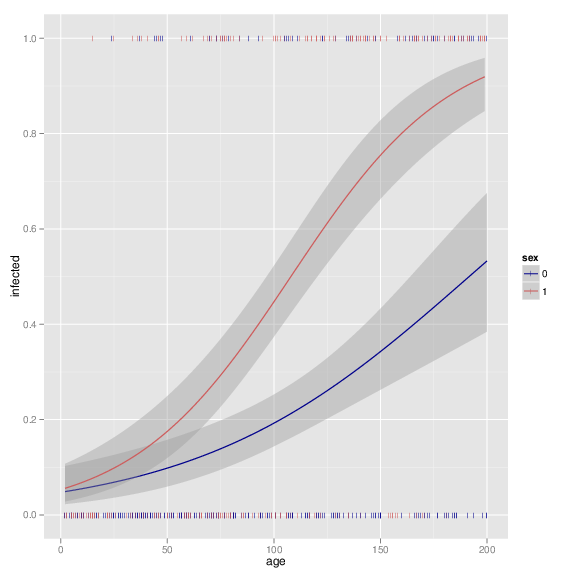
\includegraphics[width=11.5cm]{binancova1.png}
\end{center}
\end{frame}


\begin{frame}[fragile]\frametitle{Exercise}
Try to reproduce the plot! Hints:
  \begin{enumerate}
  \item set up a ggplot object, think about the aesthetics (\texttt{aes()}). Which quality of the graph you wanna set to which variable?
  \item begin with the lines (\texttt{geom\_smooth()})
  \item add the points (\texttt{geom\_jitter()}; do not think about the symbols in the first place; try to adjust the width and height appropriately)
  \item change the colour of the lines and points (\texttt{scale\_colour\_manual()}); I used midnightblue for male and deeppink for female
  \item change the symbols (\texttt{scale\_shape\_manual()}); use
\begin{verbatim}
    values = c("male" = "\u2642","female" = "\u2640"))
\end{verbatim}
     as values
  \item set the axes titles
  \item change to text of the y axis to percentage
  \item etc
  \end{enumerate}
\end{frame}



% \section{GLMs and Count Data}

% \begin{frame}[fragile]\frametitle{Count Data}
% \begin{itemize}
% \item a great deal of the data collected is in the form of counts
% \item for example:
%   \begin{itemize}
%   \item number of individuals that died
%   \item number of firms going
%   \item bankrupt, the number of days of frost, 
%   \item the number of red blood cells on a microscope slide, and the 
%   \item number of craters in a sector of lunar landscape
%   \end{itemize}
% \item with count data, the number 0 often appears as a value of the response (zero inflated data)
% \end{itemize}
% \end{frame}

% \begin{frame}[fragile]\frametitle{Count Data}
% \begin{itemize}
% \item we must consider a different cases in dealing with data on frequencies: cases
%   \begin{itemize}
%   \item   where we count how many
% times something happened, but we have no way of knowing how often it did not happen
% (e.g. lightning strikes, bankruptcies, deaths, births). 
% \item count data on proportions, where we know the number doing a particular thing, but also the number
% not doing that thing (e.g. the proportion dying, sex ratios at birth, proportions of different
% groups responding to a questionnaire)
%   \end{itemize}
% \end{itemize}
% \end{frame}

% \begin{frame}[fragile]\frametitle{A Poisson Regression}
%   \begin{itemize}
%   \item The following example has a count (the number of reported cancer cases per year per clinic) as the response variable
%   \item and a single continuous explanatory variable (the distance from a nuclear plant to the clinic in km). 
%   \item The question is whether or not proximity to the reactor affects the number of cancer cases.\small
% \begin{verbatim}
% > cancer <- read.table("clusters.txt",header=T)
% > head(cancer)
%   Cancers Distance
% 1       0 11.46952
% 2       0 66.55395
% 3       0 47.46230
% 4       0 48.38129
% 5       0 73.76534
% 6       0 70.57555
% \end{verbatim}
%   \end{itemize}
% \end{frame}


% \begin{frame}[fragile]\frametitle{Count Data}
%   \begin{itemize}
%   \item look at a barplot (cut the \texttt{Distance} variable in ten classes) and a scatter plot
%   \end{itemize}
%   \begin{columns}
%     \begin{column}{0.5\textwidth}
% \begin{center}
% 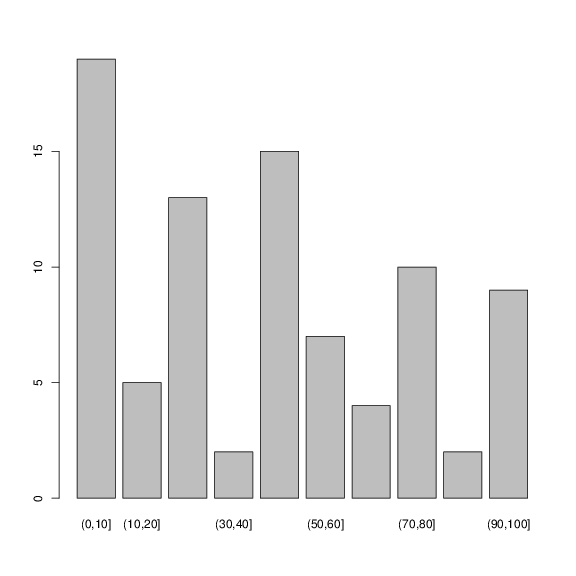
\includegraphics[width=4.5cm]{cancerdist.png}
% \end{center}
%     \end{column}
%     \begin{column}{0.5\textwidth}
% \begin{center}
% 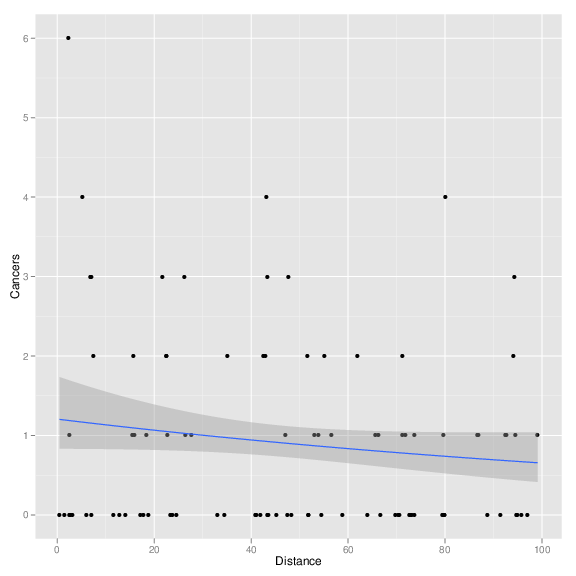
\includegraphics[width=4.5cm]{cancerdist2.png}
% \end{center}
%     \end{column}
%   \end{columns}

% \end{frame}

% \begin{frame}[fragile]\frametitle{Count Data}
%   \begin{itemize}
%   \item There seems to be a downward trend in cancer cases with distance. But is the trend significant?\footnotesize
% \begin{verbatim}
% > m <- glm(Cancers~Distance,family=poisson,data=cancer)
% > summary(m)
% Call:
% glm(formula = Cancers ~ Distance, family = poisson, 
%                                      data = cancer)

% Deviance Residuals: 
%     Min       1Q   Median       3Q      Max  
% -1.5504  -1.3491  -1.1553   0.3877   3.1304  
% Coefficients:
%              Estimate Std. Error z value Pr(>|z|)  
% (Intercept)  0.186865   0.188728   0.990   0.3221  
% Distance    -0.006138   0.003667  -1.674   0.0941 .
% (Dispersion parameter for poisson family taken to be 1)

%     Null deviance: 149.48  on 93  degrees of freedom
% Residual deviance: 146.64  on 92  degrees of freedom
% AIC: 262.41
% \end{verbatim}
%   \end{itemize}
% \end{frame}


% \begin{frame}[fragile]\frametitle{Count Data}
%   \begin{itemize}
%   \item The trend does not look to be significant, but look at the residual deviance:
%   \item It is assumed that this is the same as the residual degrees of freedom (because the errors are supposed to be Poisson distributed) 
%   \item this indicates that we have overdispersion (extra, unexplained variation in the response). 
%   \item we compensate for the overdispersion by refitting the model using quasi-Poisson rather than Poisson errors
%   \end{itemize}
% \end{frame}

% \begin{frame}[fragile]\frametitle{Count Data}
%   \begin{itemize}
% \item the refitted model\footnotesize
% \begin{verbatim}
% > m <- glm(Cancers~Distance,family=quasipoisson,data=cancer)
% > summary(m)
% Call:
% glm(formula = Cancers ~ Distance, 
%                family = quasipoisson, data = cancer)
% Deviance Residuals: 
%     Min       1Q   Median       3Q      Max  
% -1.5504  -1.3491  -1.1553   0.3877   3.1304  

% Coefficients:
%              Estimate Std. Error t value Pr(>|t|)
% (Intercept)  0.186865   0.235364   0.794    0.429
% Distance    -0.006138   0.004573  -1.342    0.183

% (Dispersion parameter for quasipoisson family 
%                                  taken to be 1.555271)
%     Null deviance: 149.48  on 93  degrees of freedom
% Residual deviance: 146.64  on 92  degrees of freedom
% \end{verbatim}
%   \end{itemize}
% \end{frame}

% \begin{frame}[fragile]\frametitle{Interpreting the Coefficients}
%   \begin{itemize}
%   \item the estimates remained the same, but the p-vals changed
%   \item so there is no compelling evidence to support the existence of a trend in cancer incidence with distance
% from the nuclear plant (this is a completely made up example, neither considering varying population nor clinic density)
%   \end{itemize}
% \end{frame}


% \begin{frame}[fragile]\frametitle{Interpreting the Coefficients}
%   \begin{itemize}
%   \item if you use glms with Poisson errors, the default link function is \texttt{log}
%   \item so the parameter estimates and the predictions from the model (the ‘linear predictor’) are in logs, and need to be antilogged
%   \item so we have the following following formula for our model
% $$\mbox{count}=\exp{(0.186865 - 0.006138 \cdot \mbox{Distance})}$$
%   \item antilog the intercept:
% \begin{verbatim}
%   > exp(coef(m)[1])
% (Intercept) 
%    1.205464 
% \end{verbatim}
% \item get 1.2 expected cases at a distance of zero
%   \end{itemize}
% \end{frame}

% \begin{frame}[fragile]\frametitle{Interpreting the Coefficients}
%   \begin{itemize}
% \item the slope for \texttt{Distance} is a bit easier to interpret than with a logit link
% \begin{verbatim}
% > exp(coef(m)[2])
%  Distance 
% 0.9938805 
% \end{verbatim}
% means that for every additional km distance you get 0.006 less cancer cases  (it is nicer to say for every 10 km the expected count of cancer cases decreases by 6\%)
%   \end{itemize}
% \end{frame}

% \begin{frame}[fragile]\frametitle{Interpreting the Coefficients}
%   \begin{itemize}
% \item again, the \texttt{effects} package is very helpful to give an overview \small
% \begin{verbatim}
% > allEffects(m,xlevels=list(Distance=seq(0,100,by=10))
% + )
%  model: Cancers ~ Distance

%  Distance effect
% Distance
%         0        10        20        30 
% 1.2054642 1.1336940 1.0661968 1.0027182 
%        40        50        60        70
% 0.9430189 0.8868740 0.8340718 0.7844133
%        80        90       100 
% 0.7377114 0.6937900 0.6524835 
% \end{verbatim}
%   \end{itemize}
% \end{frame}

% \begin{frame}[fragile]\frametitle{Interpreting the Coefficients}
%   \begin{itemize}
%   \item now the effect plot and the (non-significant) fitted line can be drawn
%   \end{itemize}
% \begin{center}
% 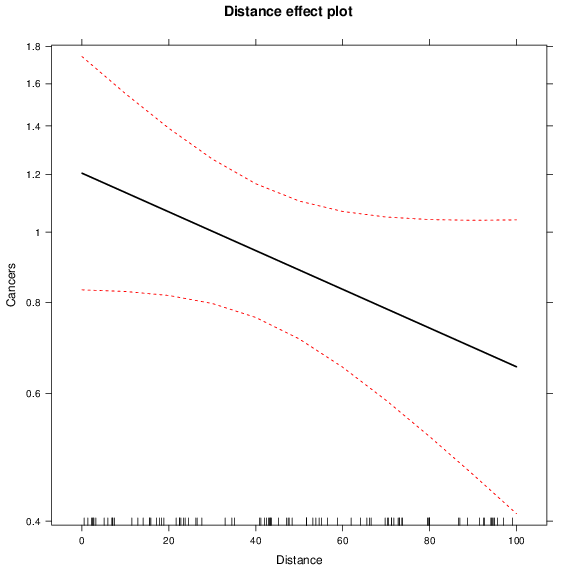
\includegraphics[width=6cm]{cancerdist3.png}
% \end{center}
% \end{frame}

% \begin{frame}[fragile]\frametitle{Interpreting the Coefficients}
% \begin{center}
% 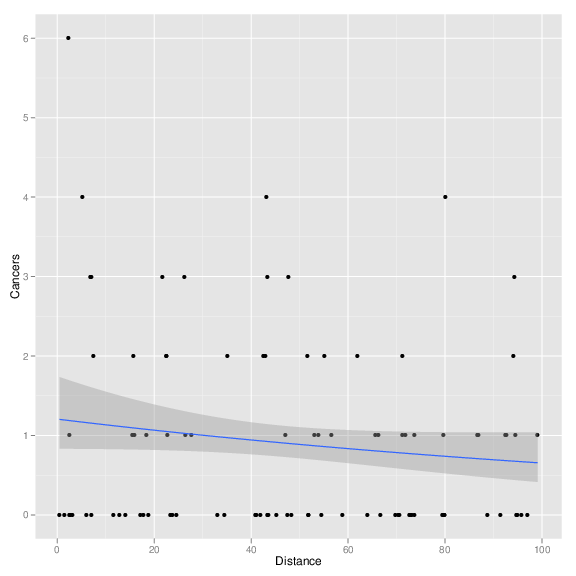
\includegraphics[width=6cm]{cancerdist2.png}
% \end{center}
% \end{frame}

% \begin{frame}[fragile]\frametitle{Anova with Count Data}
% \begin{itemize}
% \item next example the response variable is a count of infected blood cells per $\mbox{mm}^2$ on microscope slides prepared from randomly selected individuals
% \item explanatory variables are smoker (logical, yes or no)
% \item and body mass score (three levels, normal, overweight, obese)
% \item so we fit the following model (including the interaction term)\tiny
% \end{itemize}
% \end{frame}


% \begin{frame}[fragile]\frametitle{Anova with Count Data}
% \footnotesize
% \begin{verbatim}
% > m <- glm(cells~smoker*weight,family=poisson,data=cells)
% > summary(m)
% Call:
% glm(formula = cells ~ smoker * weight, family = poisson, data = cells)
% Deviance Residuals: 
%     Min       1Q   Median       3Q      Max  
% -2.6511  -1.1742  -0.9148   0.5533   3.6436  
% Coefficients:           Estimate Std. Error z value Pr(>|z|)    
% (Intercept)             -0.8712     0.1302  -6.692 2.20e-11 ***
% smokerTRUE               0.8224     0.1833   4.486 7.27e-06 ***
% weightobese              0.4993     0.1671   2.987 0.002817 ** 
% weightover               0.2618     0.1866   1.404 0.160465    
% smokerTRUE:weightobese   0.8063     0.2296   3.511 0.000446 ***
% smokerTRUE:weightover    0.4935     0.2546   1.939 0.052548 .  

% (Dispersion parameter for poisson family taken to be 1)
%     Null deviance: 1052.95  on 510  degrees of freedom
% Residual deviance:  792.85  on 505  degrees of freedom
% AIC: 1318.5
% \end{verbatim}
% \end{frame}




% \begin{frame}[fragile]\frametitle{Anova with Count Data}
%   \begin{itemize}
%   \item again we see overdispersion (residual deviance $>$ degrees of freedom)
%   \item we compensate by refitting the model using quasi-Poisson errors
%   \end{itemize}
% \end{frame}


% \begin{frame}[fragile]\frametitle{Anova with Count Data}
% \footnotesize
% \begin{verbatim}
% > m <- glm(cells~smoker*weight,family=quasipoisson,data=cells)
% > summary(m)
% Call:
% glm(formula = cells ~ smoker * weight, family = quasipoisson, 
%     data = cells)
% Deviance Residuals: 
%     Min       1Q   Median       3Q      Max  
% -2.6511  -1.1742  -0.9148   0.5533   3.6436  
% Coefficients:
%                        Estimate Std. Error t value Pr(>|t|)    
% (Intercept)             -0.8712     0.1760  -4.950 1.01e-06 ***
% smokerTRUE               0.8224     0.2479   3.318 0.000973 ***
% weightobese              0.4993     0.2260   2.209 0.027598 *  
% weightover               0.2618     0.2522   1.038 0.299723    
% smokerTRUE:weightobese   0.8063     0.3105   2.597 0.009675 ** 
% smokerTRUE:weightover    0.4935     0.3442   1.434 0.152226    

% (Dispersion parameter for quasipoisson family taken to be 1.827927)
% \end{verbatim}
% \end{frame}

% \begin{frame}[fragile]\frametitle{Interpreting the Coefficients}\footnotesize
%   \begin{itemize}
% \item remember poisson has log as link so
% \begin{verbatim}
% > exp(coef(m)[1])
% (Intercept) 
%   0.4184397 
% \end{verbatim}
% is the expected count of infected blood cells for a normal weighted non-smoker
% \item all the other estimates are interpretable as factors (because of the log link!)
% \item so a smoker has 
% \begin{verbatim}
% > exp(coef(m)[2])
% smokerTRUE 
%   2.276029 
% \end{verbatim}
% more than twice as many infected cells which is
% \begin{verbatim}
% > exp(coef(m)[1])*exp(coef(m)[2])
% (Intercept) 
%    0.952381 
% \end{verbatim}
% expected infected cells, etc. pp
%   \end{itemize}
% \end{frame}

% \begin{frame}[fragile]\frametitle{Interpreting the Coefficients}
%   \begin{itemize}
%   \item unfortunately \texttt{effect()} does not work on our model object, so we use \texttt{tapply()} (for simple models a good alternative, as soon as I remove an interaction term, or nested effects this does not work anymore)\footnotesize
% \begin{verbatim}
% > with(cells,tapply(cells,list(smoker,weight),mean))
%          normal     obese      over
% FALSE 0.4184397 0.6893939 0.5436893
% TRUE  0.9523810 3.5142857 2.0270270
% \end{verbatim}
%   \end{itemize}
% \end{frame}


% \begin{frame}[fragile]\frametitle{Interpreting the Coefficients}
%   \begin{itemize}
%   \item for visualization we use barplot with errorbars indicating the standard error
%   \end{itemize}
% \begin{center}
% 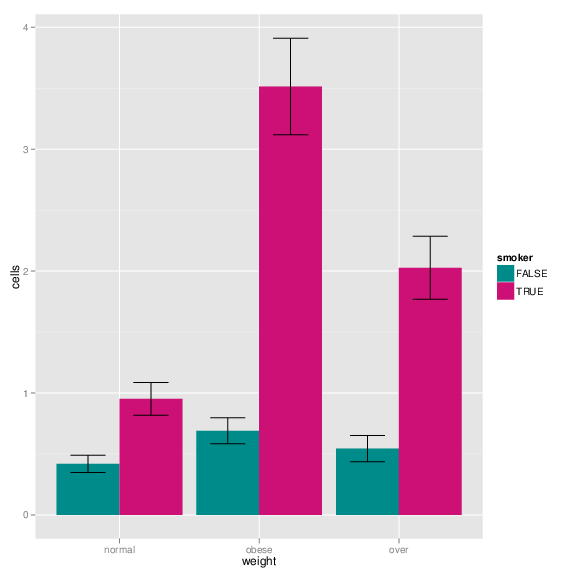
\includegraphics[width=7cm]{obesesmokers.png}
% \end{center}
% \end{frame}

% \begin{frame}[fragile]\frametitle{Ancova with Count Data}
%   \begin{itemize}
%   \item last example: analysis of covariance
%   \item response is a count of the number of plant species on plots 
%   \item that have different biomass (a continuous explanatory variable) and
%   \item different soil pH (a categorical variable with three levels: high, mid and low)
% \begin{verbatim}
% > species<-read.table("species.txt",header=T)
% > head(species)
%     pH   Biomass Species
% 1 high 0.4692972      30
% 2 high 1.7308704      39
% 3 high 2.0897785      44
% 4 high 3.9257871      35
% 5 high 4.3667927      25
% 6 high 5.4819747      29
% \end{verbatim}
%   \end{itemize}
% \end{frame}

% \begin{frame}[fragile]\frametitle{Ancova with Count Data}
%   \begin{itemize}
%   \item this time we begin with a scatter plot\small
% \begin{verbatim}
% p <- ggplot(species,aes(x=Biomass,y=Species,
% +                         shape=pH,colour=pH)) +
%      geom_point()
% \end{verbatim}
%   \end{itemize}
% \begin{center}
% 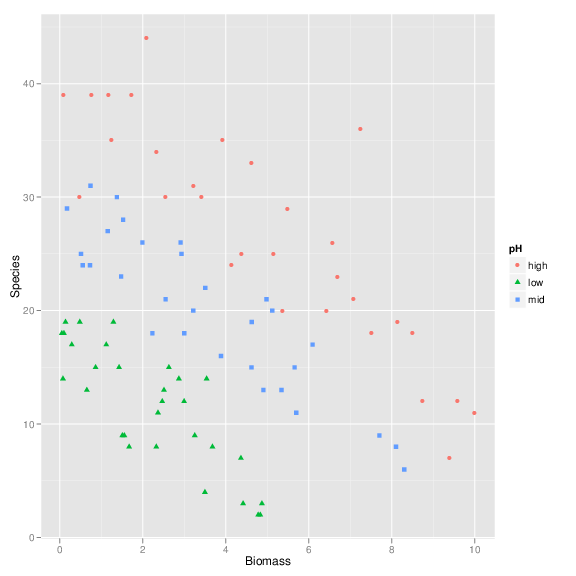
\includegraphics[width=4.5cm]{species.png}
% \end{center}
% \end{frame}

% \begin{frame}[fragile]\frametitle{Ancova with Count Data}
%   \begin{itemize}
% \item we see: number of species declines with Biomass
% \item soil pH has a big effect on Species 
% \item Does the slope of the relationship between Species and Biomass depend
% on pH?
%   \end{itemize}
% \end{frame}


% \begin{frame}[fragile]\frametitle{Ancova with Count Data}
%   \begin{itemize}
%   \item define the model and look at the summary\small
% \begin{verbatim}
% > m <- glm(Species~Biomass*pH,family=poisson,data=species)
% > summary(m)
% ...
% Coefficients:
%               Estimate Std. Error z value Pr(>|z|)    
% (Intercept)    3.76812    0.06153  61.240  < 2e-16 ***
% Biomass       -0.10713    0.01249  -8.577  < 2e-16 ***
% pHlow         -0.81557    0.10284  -7.931 2.18e-15 ***
% pHmid         -0.33146    0.09217  -3.596 0.000323 ***
% Biomass:pHlow -0.15503    0.04003  -3.873 0.000108 ***
% Biomass:pHmid -0.03189    0.02308  -1.382 0.166954    
% ...
% \end{verbatim}
%   \end{itemize}
% \end{frame}

% \begin{frame}[fragile]\frametitle{Ancova with Count Data}
%   \begin{itemize}
%   \item test for the need for different slopes by comparing this maximal model (with
% six parameters) with a simpler model with different intercepts but the same slope
% \begin{verbatim}
% > m2 <- glm(Species~Biomass+pH,
% +                 family=poisson,data=species)
% > anova(m,m2,test="Chi")
% Analysis of Deviance Table

% Model 1: Species ~ Biomass * pH
% Model 2: Species ~ Biomass + pH
%   Resid. Df Resid. Dev Df Deviance  Pr(>Chi)    
% 1        84     83.201                          
% 2        86     99.242 -2   -16.04 0.0003288 ***
% \end{verbatim}
% \item AIC: m: 514.4; m2: 526.4 
%   \end{itemize}
% \end{frame}

% \begin{frame}[fragile]\frametitle{Ancova with Count Data}
%   \begin{itemize}
%   \item slopes are very significantly different $p = 0.00033$ , so it is justified to retain the more complicated model
%   \item finally, we have a look on the effects and then draw the fitted lines through the scatterplot using the plot object \texttt{p} from above
%   \end{itemize}\small
% \begin{verbatim}
% > allEffects(m,xlevels=list(Biomass=1:10))
%  model: Species ~ Biomass * pH
%  Biomass*pH effect
%        pH
% Biomass     high       low       mid
%      1  38.89998 14.737487 27.048707
%      2  34.94810 11.338867 23.538030
%      3  31.39769  8.724005 20.483007
%      4  28.20797  6.712158 17.824498
%      5  25.34229  5.164264 15.511039
%      6  22.76775  3.973330 13.497847
%      ....
% \end{verbatim}
% \end{frame}

% \begin{frame}[fragile]\frametitle{Ancova with Count Data}
%   \begin{columns}
%     \begin{column}{0.5\textwidth}
% \begin{center}
% 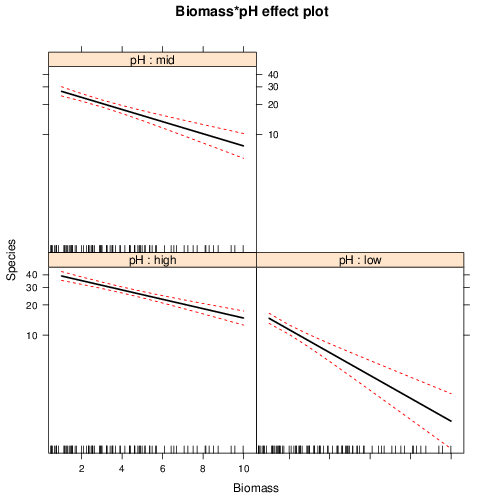
\includegraphics[width=4.5cm]{species2.png}
% \end{center}
%     \end{column}
%     \begin{column}{0.5\textwidth}
% \begin{center}
% 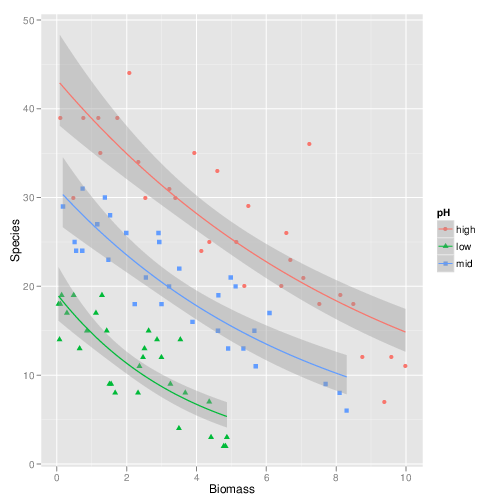
\includegraphics[width=4.5cm]{species3.png}
% \end{center}
%     \end{column}
%   \end{columns}
% \end{frame}

% \section{Count Data on Proportions}
% \begin{frame}[fragile]\frametitle{Proportion Data}
%   \begin{itemize}
%   \item For comparisons of one binomial proportion with a constant, use \texttt{binom.test()}
%   \item For comparison of two samples of proportion data, use \texttt{prop.test()}
%   \item The use of GLMs on proportion data is for complex models
%   \end{itemize}
% \end{frame}

% \begin{frame}[fragile]\frametitle{GLMs \& Proportion Data}
%   \begin{itemize}
%   \item uses also logit as link function and binomial error distribution
%   \item if there is overdispersion use quasibinomial to compensate
%   \item fitted values are counts
%   \item we have seen one example so far: in the challenger example we have already used the responds variable in form of a proportion
%   \end{itemize}
% \end{frame}

% \begin{frame}[fragile]\frametitle{GLMs \& Proportion Data}
%   \begin{itemize}
%   \item we use an example concerning sex ratios in insects as response and
%   \item population density as explanatory variable
%   \item so load the data and fit the model
% \begin{verbatim}
% > numbers <-read.table("sexratio.txt",header=T)
% > head(numbers)
%   density females males
% 1       1       1     0
% 2       4       3     1
% 3      10       7     3
% 4      22      18     4
% 5      55      22    33
% 6     121      41    80
% > m <- glm(cbind(males,females)~density,
% +                  family=binomial,data=numbers)
% \end{verbatim}
%   \end{itemize}
% \end{frame}

% \begin{frame}[fragile]\frametitle{GLMs \& Proportion Data}\footnotesize
% \begin{verbatim}
% > summary(m)
% Call:
% glm(formula = cbind(males, females) ~ density, family = binomial, 
%     data = numbers)

% Deviance Residuals: 
%     Min       1Q   Median       3Q      Max  
% -3.4619  -1.2760  -0.9911   0.5742   1.8795  

% Coefficients:
%              Estimate Std. Error z value Pr(>|z|)    
% (Intercept) 0.0807368  0.1550376   0.521    0.603    
% density     0.0035101  0.0005116   6.862 6.81e-12 ***

% (Dispersion parameter for binomial family taken to be 1)
%     Null deviance: 71.159  on 7  degrees of freedom
% Residual deviance: 22.091  on 6  degrees of freedom
% AIC: 54.618
% \end{verbatim}
% \end{frame}

% \begin{frame}[fragile]\frametitle{GLMs \& Proportion Data}
%   \begin{itemize}
%   \item the residual deviance is larger than the residual degrees of freedom
%   \item because it is something like a growth process we try a log transformation (before using quasibinomial family)\tiny
% \begin{verbatim}
% > m <- glm(cbind(males,females)~log(density),
% +                           family=binomial,data=numbers)
% > summary(m)
% Call:
% glm(formula = cbind(males, females) ~ log(density), 
%                    family = binomial, data = numbers)
% Deviance Residuals: 
%     Min       1Q   Median       3Q      Max  
% -1.9697  -0.3411   0.1499   0.4019   1.0372  

% Coefficients:
%              Estimate Std. Error z value Pr(>|z|)    
% (Intercept)  -2.65927    0.48758  -5.454 4.92e-08 ***
% log(density)  0.69410    0.09056   7.665 1.80e-14 ***

%     Null deviance: 71.1593  on 7  degrees of freedom
% Residual deviance:  5.6739  on 6  degrees of freedom
% AIC: 38.201
% \end{verbatim}
%   \end{itemize}
% \end{frame}

% \begin{frame}[fragile]\frametitle{GLMs \& Proportion Data}
%   \begin{itemize}
%   \item the transformation caused a welcome decrease in the residual deviance
%   \item we conclude that the proportion of animals that are males increases significantly with
% increasing density, and 
% \item that the logistic model is linearized by logarithmic transformation of the explanatory variable
%   \end{itemize}
% \end{frame}

% \begin{frame}[fragile]\frametitle{GLMs \& Proportion Data}
% \begin{verbatim}
% ggplot(numbers, aes(x=log(density),y=males/(males+females))) +
%   geom_point() +
%   geom_smooth(method=glm,family=binomial)
% \end{verbatim}
% \begin{center}
% 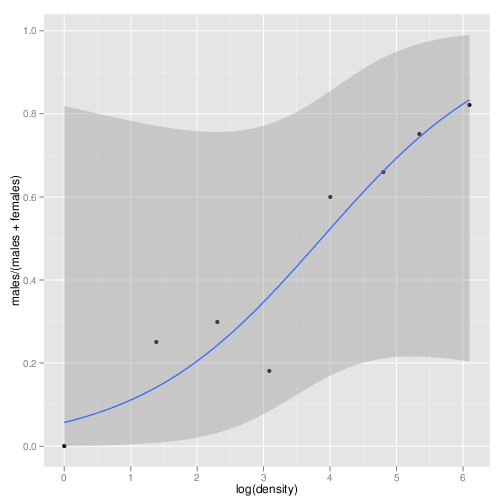
\includegraphics[width=4.5cm]{sexratio.png}
% \end{center}
% \end{frame}
